\chapter{Results and Discussion} \label{Results and discussion}

%aj - result in current form will not be accepatable. Make new section for each of number 1-5. Then include some snapsot of images. 

% image of the videos 
The results of this thesis are documented in this Youtube playlist \cite{youtube_playlist_results}. The playlist consists of five videos. 

\subsection{TB autonompous driving}
The first video, "TB w Nav2" shows TB3 driving autonomously using ROS2 Galactic, Nav2, and SLAM Toolbox. An external computer is used to set the initial position and goals from Rviz. Nav2 works well with TB3, but the system could benefit from a 3D LiDAR so it could sense obstacles below the LiDAR. 
\begin{figure}[H]
  \centering
  \begin{minipage}[b]{0.5\textwidth}
    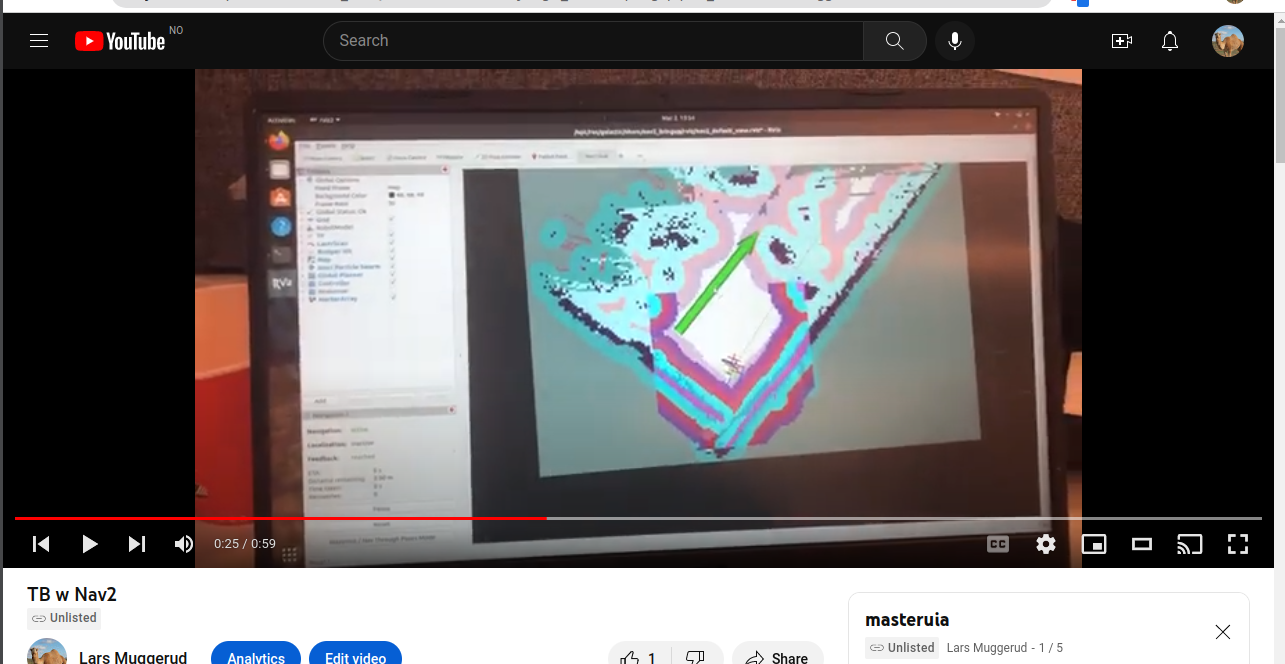
\includegraphics[width=\textwidth]{Figures/YouTube/TB w Nav2 1.png}
    \caption{Rviz is used to interact with Nav2 running on the TB3.}
    \label{fig:TB w Nav2 1.png}
  \end{minipage}
  \hfill
  \begin{minipage}[b]{0.49\textwidth}
    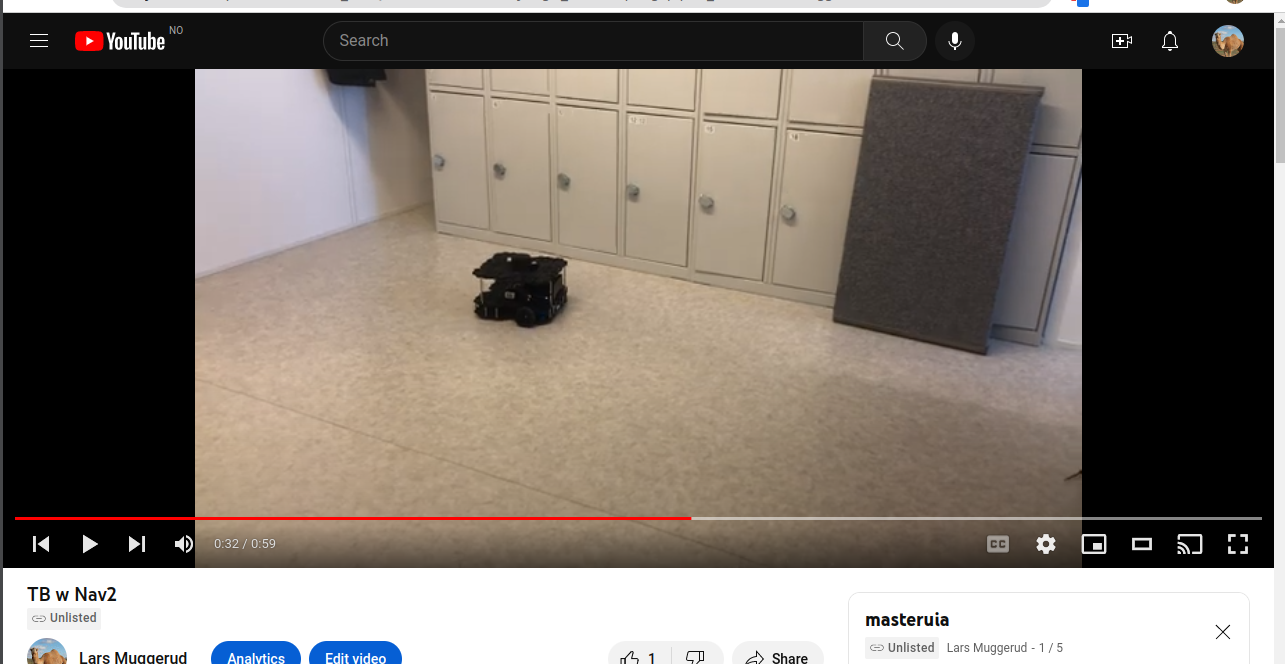
\includegraphics[width=\textwidth]{Figures/YouTube/TB w Nav2 2.png}
    \caption{TB3 driving autonomous with Nav2.}
    \label{fig:TB w Nav2 2}
  \end{minipage}
\end{figure}

\subsection{Husky autonomous driving}
"Nav2SLAM 2etg" \label{Nav2SLAM 2etg} is showing Husky driving autonomous using ROS2 Foxy and Galactic, Nav2, SLAM Toolbox. An external computer is used to set the initial position and goals from Rviz. 

\begin{figure}[H]
    \centering
    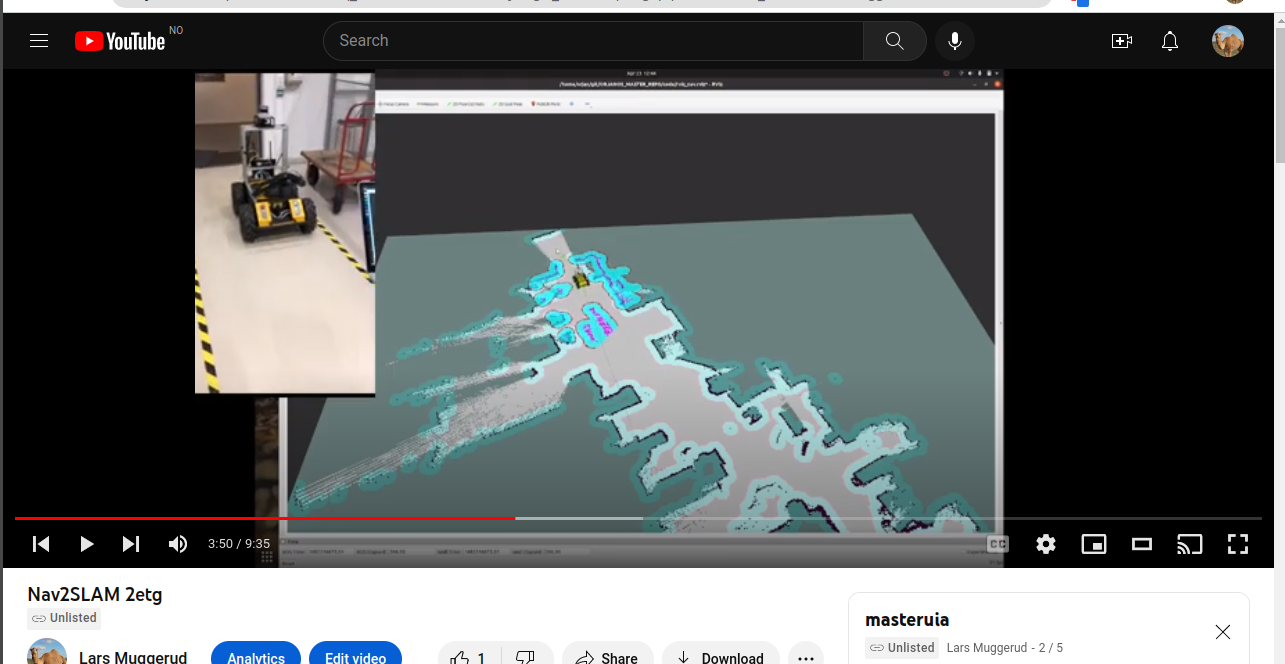
\includegraphics[width=\textwidth]{Figures/YouTube/Nav2SLAM 2etg.png}
    \caption{Husky driving autonomous with Nav2, Rviz is used to interact with Nav2.}
    \label{fig:Nav2SLAM 2etg}
\end{figure}

At \href{https://youtu.be/JiTbKtXq_GY?t=65}{1:05}, the husky struggles with navigating. This could be caused by the range of the LiDAR, skidding wheels, the cameraman walking behind the Husky, or a combination. 
Skidding problems can be solved by using a different robot with, for example, omnidirectional turning. The problem with skidding often occurs when Nav2 to goes into recovery mode, which is started when Nav2 is uncertain of the position of the robots. Nav2 commands the robot to spin around its own axes to recover the position estimate, but whit a skid-turning robot, turning creates uncertainty. It seems that Nav2 gains information by rotating the even for a skid-turning robot but not as much as an omnidirectional robot. Spin around its own axes seems like a safe way to recover, but maybe other alternatives of recovery for skid-turning robots this has not been looked into. 
The range of the Ouster LiDAR cant be changed, but the placement can. During this thesis, the LiDAR has been placed high up in front, and it has been observed that this works poorly for indoor navigation. The Husky has been tested with the LiDAR placed lower, and this improves the ability to see relevant obstacles. The placement of the LiDAR has a great impact on autonomous navigation but has not been properly tested in this thesis. Placing the LiDAR lower will cause it to see more obstacles on the ground. The LiDAR can also be placed further back, increasing the distance to the front of the Husky, and making the LiDAR see obstacles closer to the front. If the LiDAR is too far back, it will loos information from the obstacles on the ground. Close-range sensors could also be added to the front to detect where the LiDAR can not. 
The position of the LiDAR and the steering method is important for navigation and differ between navigation tasks, such as indoor vs. outdoor. This should maybe have been looked more into.

    It should be mentioned that the two robots are also able to drive on a pre-made map with Nav2 localization. They can also make a map when controlled manually. This was not recorded and edited due to time limitations. 
\subsection{Mimic}
%include the images from that video where mimic is implemented and explain in words. done

"Mimic" \ref{Mimic} is a video showing the TB3 mimicking the Husky controlled by teleop. This shows how well ROS communicates the same message to different hardware. This shows that mimic can be used simultaneous breaking or lane switching, and could be implemented as a part of a bigger platooning system. 

\begin{figure}[H]
    \centering
    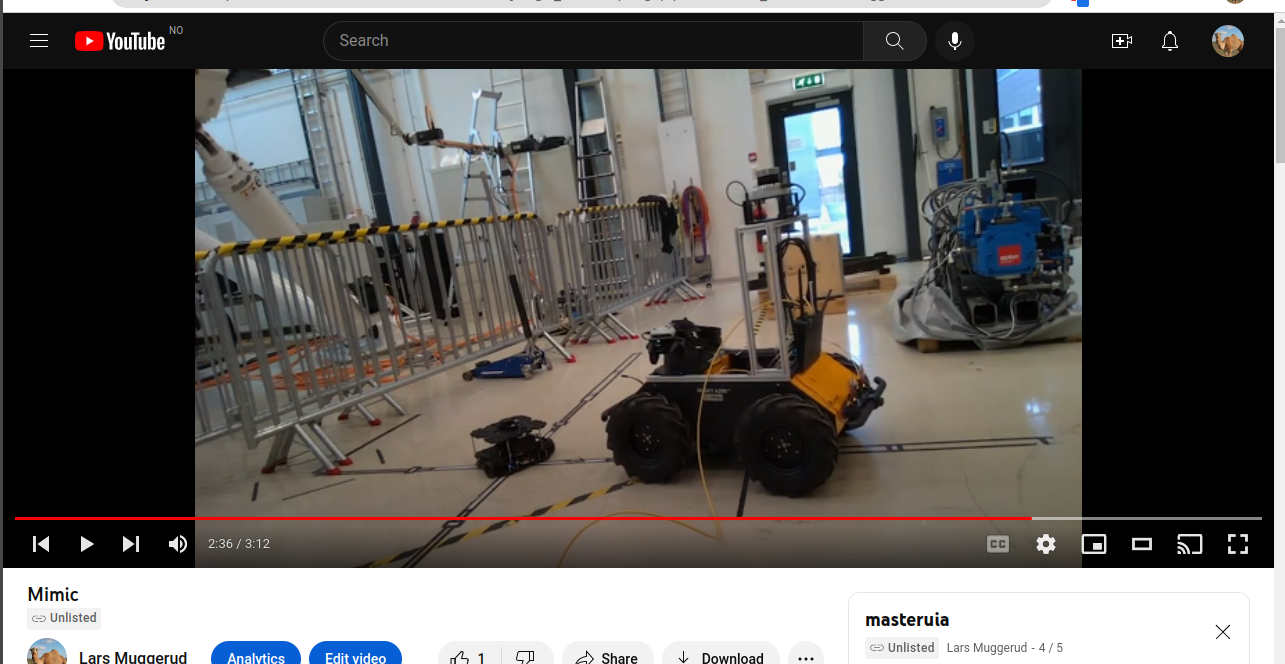
\includegraphics[width=\textwidth]{Figures/YouTube/Mimic.png}
    \caption{TB3 and Husky mirroring etch other in the Mimic video}
    \label{fig:Mimic}
\end{figure}

\subsection{Time delay}
% include the images from that video where time delay is implemented and explain in words. LM done

"TimeDelayTest" is video where the Husky is driven by teleop and the TB3 follows using the Time Delay algorithm \ref{Time delay}. 

\begin{figure}[H]
  \centering
  \begin{minipage}[b]{0.5\textwidth}
    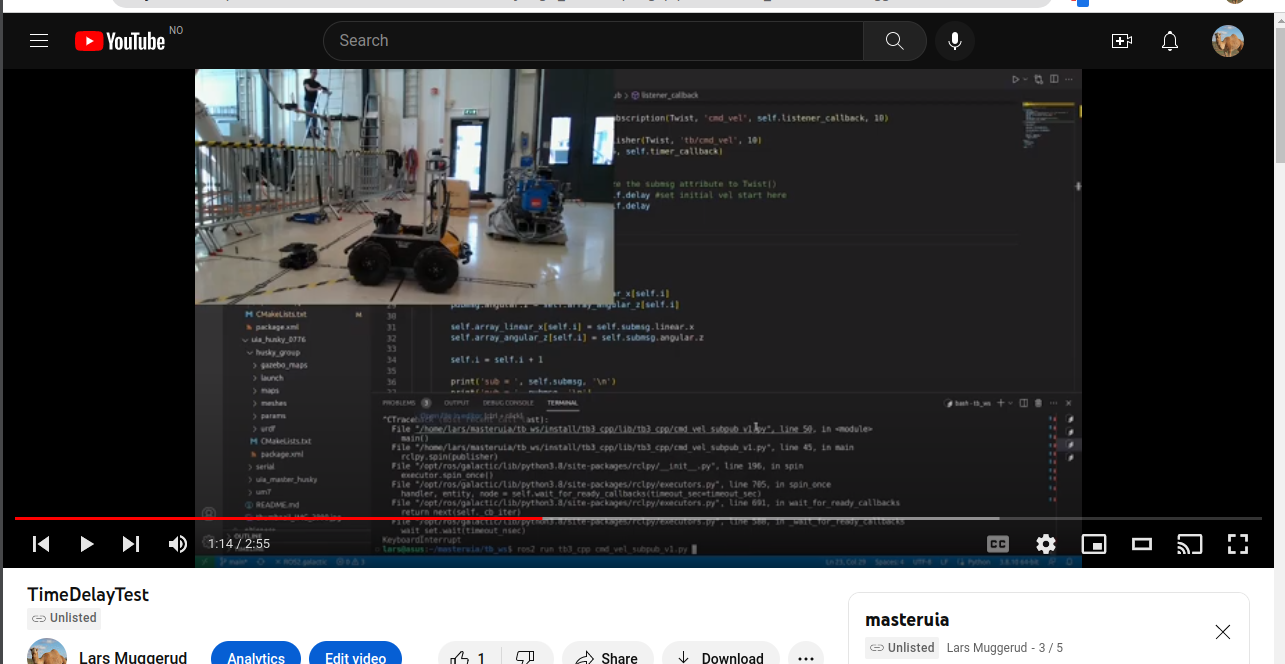
\includegraphics[width=\textwidth]{Figures/YouTube/TimeDelayTest.png}
    \caption{Photo of the TB3 and Husky are lined up 1 meter apart ready to drive.}
    \label{fig:TB w Nav2 1.png}
  \end{minipage}
  \hfill
  \begin{minipage}[b]{0.49\textwidth}
    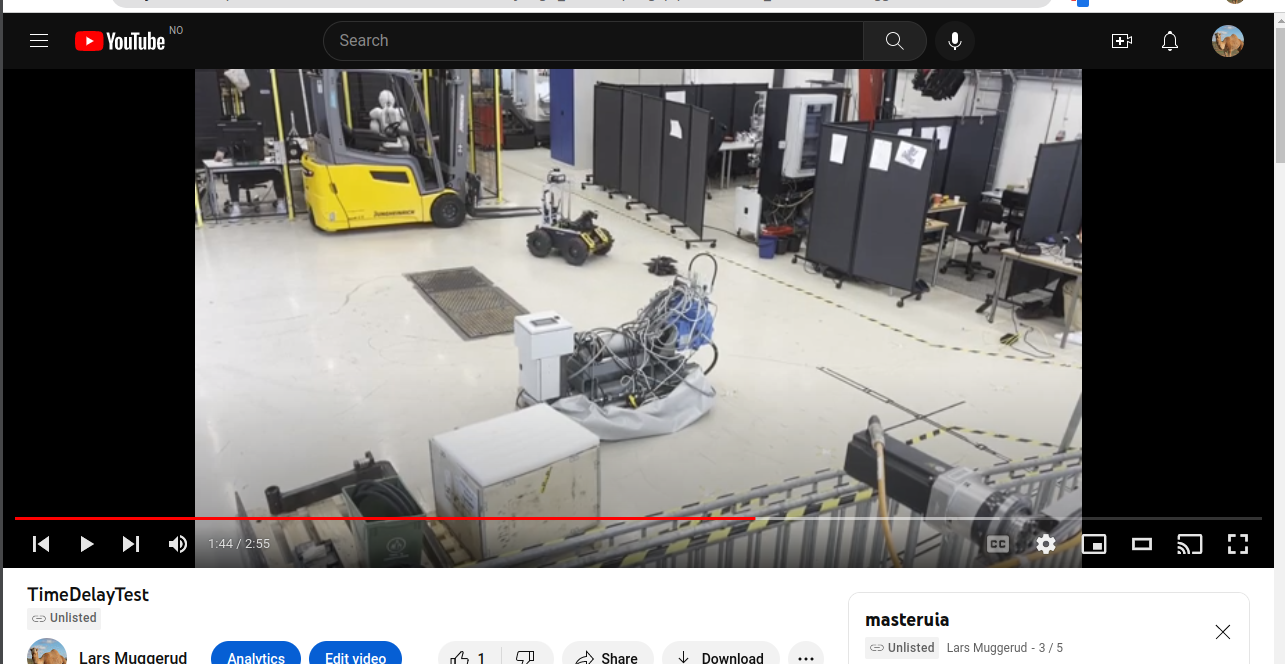
\includegraphics[width=\textwidth]{Figures/YouTube/TimeDelayTest_2.png}
    \caption{TB3 flowing the Husky, which is controlled by teleop.}
    \label{fig:TB w Nav2 2}
  \end{minipage}
\end{figure}

    
"HuskyNav2 TBsubpub" \label{HuskyNav2 TBsubpub} is showing Husky driving autonomously using ROS2 Foxy and Galactic, Nav2, SLAM Toolbox while the TB3 is following using the Time Delay algorithm \ref{Time delay}. The algorithm is not suited for autonomous platooning. In theory, the follower should copy the leader just later in time. This means if the leader stops for more than the time delay follower and leader will collide. Even though, in theory, the same velocity command should create the same movement for two different robots, it does not accomplish this in practice. The errors will accumulate over time, and the follower will drift out of the path. 

\begin{figure}[H]
  \centering
  \begin{minipage}[b]{0.5\textwidth}
    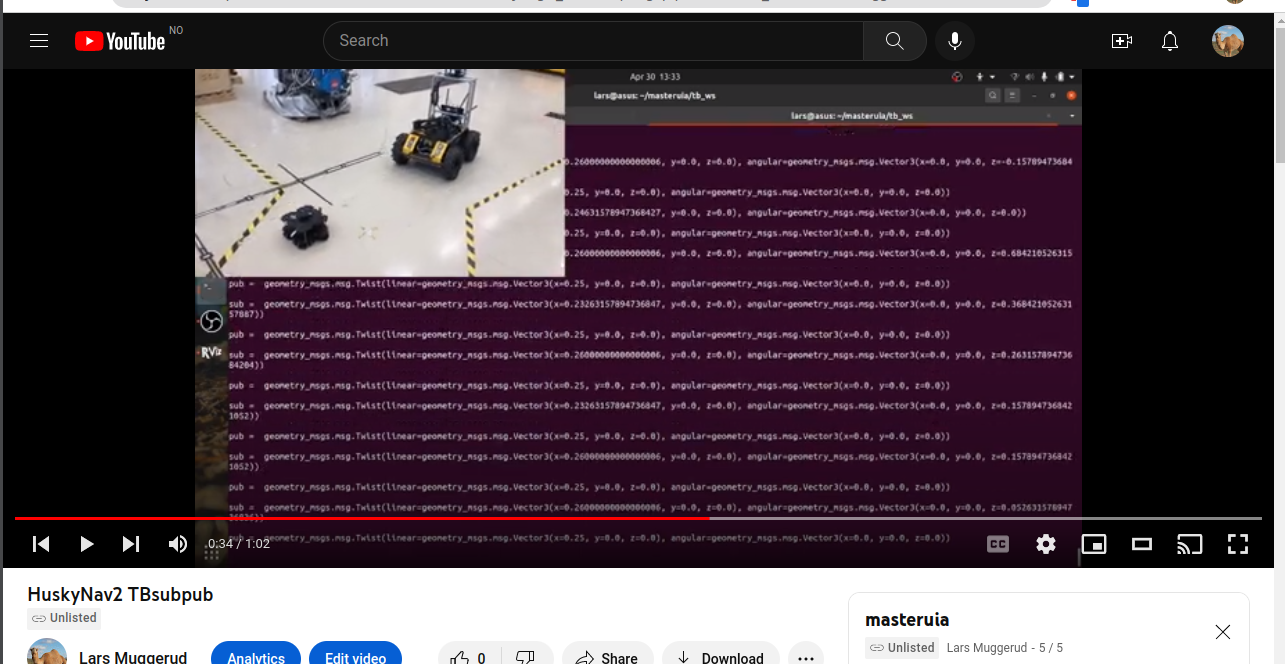
\includegraphics[width=\textwidth]{Figures/YouTube/HuksyNav2 TBsubpub.png}
    \caption{Husky driving with Nav2 and TB3 following. In the terminal the platooning algorithm is printing velocity commands received from the Husky and the ones sent to the TB3.}
    \label{fig:TB w Nav2 1.png}
  \end{minipage}
  \hfill
  \begin{minipage}[b]{0.49\textwidth}
    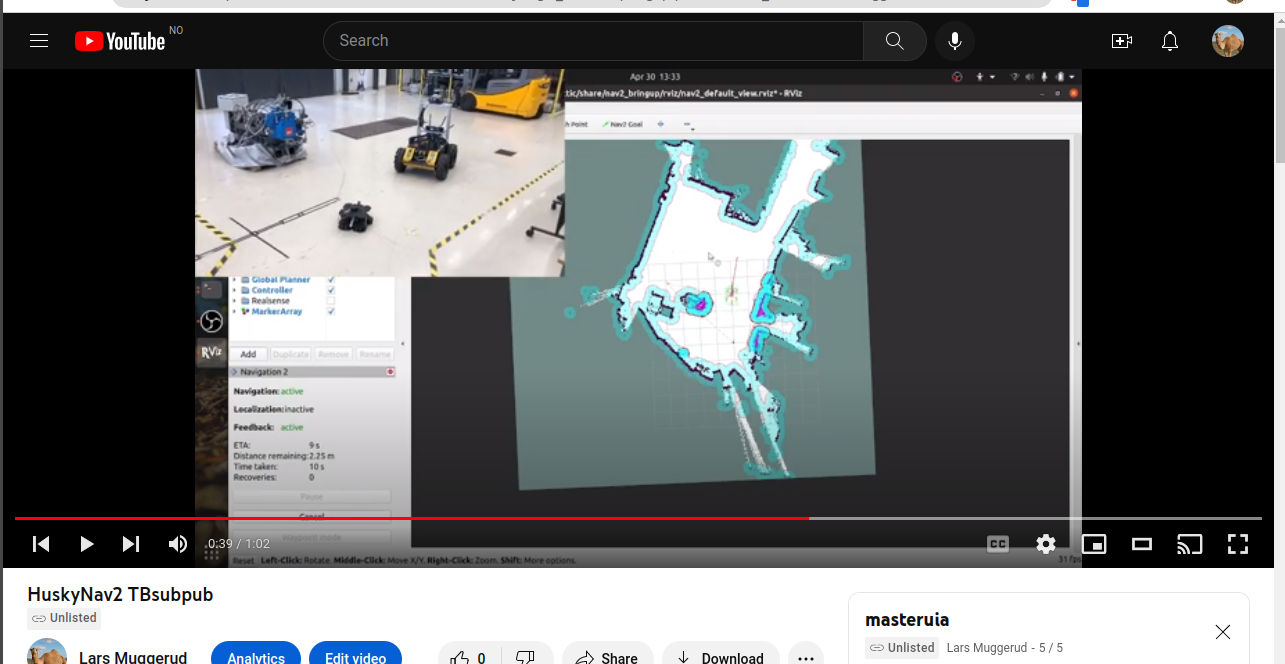
\includegraphics[width=\textwidth]{Figures/YouTube/HuskyNav2 TBsubpub2.png}
    \caption{Husky driving with Nav2 and TB3 following. Rviz is used to send goal positions to Nav2.}
    \label{fig:TB w Nav2 2}
  \end{minipage}
\end{figure}

    
The Time Delay algorithm can be improved with more information in the "subpub" node. The node can subscribe to odometry of Husky and TB3, and use this information to calculate the offset of where the TB3 is and where it should be. When Husky drives with Nav2, the topic \topic{/path} can be used to improve the awareness of where the TB3 should be. Potentially, LiDAR data can also be used and the algorithm could be improved forever. Continuing to enhance Time Delay is akin to constructing an inferior version of Nav2. Therefore the author of this thesis believes using Nav2 API \ref{Further_work_Nav2_API} is a better way to achieve autonomous platooning with ROS2. 


\paragraph{The Xavier's} has not been the focus of the thesis but is worth discussing since it's the computer of both robots. In this project, AI applications are not used which is what the Xaviers are made for. The JetPack and GPU are useless in this project. The Xavier uses ARM, and x86-64 is the most used CPU architecture. Since more people are using x86-64 there are more help and software available online. 
It could be that the Xavier is well suited for AI applications, but for future work, this thesis would recommend x86-64 CPU, no GPU, and pure Ubuntu for ROS2 projects. A GPU does not hurt but not necessary unless the PC on the robot is going to run simulations or AI. Pure Ubuntu is preferable for a more extensive community, faster updates, and less bloat. 
%aj above para LM :do you want this over or under the subsections with the videos? 

\paragraph{ROS2 Foxy and Galactic} has been used in this project. Both robots have been tested with Foxy and Galactic. From this experience, the top priority should be to choose the packages which work well for the hardware. Ideally, a common LTS (Long Term Support) ROS distribution should be used to reduce sources of error and more software and help online, but it is more important choosing packages that work well with the hardware. 
%aj above para